\PassOptionsToPackage{pdftex}{graphicx} % pdftex hack fuer graphicx
\documentclass[pdftex,hyperref=pdftex,10pt]{beamer}
\usetheme{cau}


\usepackage[utf8]{inputenc}
\usepackage[T1]{fontenc}
\usepackage[american,ngerman]{babel}
\usepackage{mathabx}



\usepackage{multicol}
\usepackage{natbib}
%% Beamer Bibliography Fix
\def\newblock{\hskip .11em plus .33em minus .07em}
\renewcommand{\bibsection}{}
% \bibliographystyle{natdin}
% \bibliographystyle{abbrvnat}
\bibliographystyle{alpha}
% \bibliographystyle{plainnat}

% listings
\usepackage{listings}
\usepackage{lstlinebgrd}
\usepackage{pgf, pgffor}
%%%%%%%%%%%%%%%%%%%%%%%%%%%%%%%%
% language specification
% for lstlistings
%
% requires setup from lstide.sty
% keywords 1 = primary keywords
% keywords 2 = secondary words and symbols to highlight
%              use alsoletter to specify additional letters for "keywords"
% keywords 3 = data types

\lstdefinelanguage{logic}{
alsoletter={},
keywords=[1]{process,condition,conditional,action,case,cases,references,start,default,send,continue,receive,subprocess,state,machine,from,to, stepwise,transition,if,then,change,with},
keywords=[2]{-, ->,this,null,true,false},
keywords=[3]{Integer,List,Collection},
string=[b]{\"},
morecomment=[l]{//},
morecomment=[s]{/*}{*/}
}

\lstdefinelanguage{types}{
alsoletter={},
keywords=[1]{communication,description,:,properties,messages,rules,interlocking,element,enumeration,state,set,
roles,statevars},
keywords=[2]{->,this,null,true,false},
keywords=[3]{Integer,List,Collection},
string=[b]{\"},
morecomment=[l]{//},
morecomment=[s]{/*}{*/}
}

\lstdefinelanguage{device}{
keywords=[1]{device, slaves, inputs, named, fetched, from, outputs, forwarded, to, deployment, bit, inverse},
keywords=[2]{ -, ->, \{, \}, \[, \], \<, \>},
string=[b]{\"},
morecomment=[l]{//},
morecomment=[s]{/*}{*/}
}

\lstdefinelanguage{deployment}{
keywords=[1]{interlocking, unit, devices, deployment, connections, tasks},
keywords=[2]{ -, ->, \{, \}, \[, \], \<, \>},
string=[b]{\"},
morecomment=[l]{//},
morecomment=[s]{/*}{*/}
}

\lstdefinelanguage{mdl}{
alsoletter={[,],:,+,-,/,*},
keywords=[1]{library,meta,model,enum,interval,measure,with},
keywords=[2]{named,-,+,:,*,/,[,],in},
keywords=[3]{ID,String,String[]},
string=[b]{\"},
}

\lstdefinelanguage{mql}{
alsoletter={},
keywords=[1]{SELECT,FROM,WHERE,AS,MEMBER,OF,GROUP,BY,ORDER,OUTPUT,EVERY,AGGREGATE,OVER,MODEL,METRIC},
keywords=[2]{max,min,average},
string=[b]{\"},
morecomment=[l]{//},
morecomment=[s]{/*}{*/}
}

\lstdefinelanguage{antlr}{
    alsoletter={:,|,;},%
    keywords=[2]{:,|,;},%                                 define the special characters
    moredelim=[s][\color{literal!50!black}\ttfamily]{'}{'},% single quotes in green
    moredelim=*[s][\color{normal}\ttfamily]{options}{\}},%  options in black (until trailing })
    morecomment=[l]{//},%                                  define // comment
    emph={STRING}
}

\lstdefinelanguage{xtext}{
    alsoletter={:,|,;},%
    keywords=[1]{import,returns,generate,as,terminal},
    keywords=[2]{:,|,;},%                                 define the special characters
    keywords=[3]{name},
    moredelim=[s][\color{literal!50!black}\ttfamily]{'}{'},% single quotes in green
    moredelim=*[s][\color{normal}\ttfamily]{options}{\}},%  options in black (until trailing })
    morecomment=[l]{//},%                                  define // comment
    emph={STRING,INT,ID}
}

%% Xtend augmented with extra colors for special example properties
\definecolor{semCommentColor}{RGB}{66, 96, 184}
\definecolor{actualTypeC}{RGB}{171,48,0}

\lstdefinelanguage{xtend}{
    language=Java,
    morekeywords={def,dispatch},
    keywordstyle=[2]\color{actualTypeC},
    morekeywords=[2]{actualType},
    morecomment=[s][\color{semCommentColor}]{/**}{*/}
}

\lstdefinelanguage{idl}{
alsoletter={=,[,],:,+,-,/,*},
keywords=[1]{package,record,default},
keywords=[2]{=},
keywords=[3]{string,long,int},
string=[b]{\"},
}

\usepackage{lstide}

\usepackage{ifthen}
\newcommand{\highlight}[1]{\textcolor{cauTF}{#1}}
\newcommand{\scite}[2][]{%
  \ifthenelse{\equal{#1}{}}{{\scriptsize{\cite{#2}}}}{{\scriptsize{\cite[#1]{#2}}}}%
}
\newcommand{\tcite}[2][]{%
  \ifthenelse{\equal{#1}{}}{{\tiny{\cite{#2}}}}{{\tiny{\cite[#1]{#2}}}}%
}

\makeatletter

%%%%%%%%%%%%%%%
%% HOTE: I don't know why this has to be between \makeatletter and \makeatother (rju)
%% Highlight lines in listings
\newcount\bt@rangea
\newcount\bt@rangeb

\newcommand\btIfInRange[2]{%
    \global\let\bt@inrange\@secondoftwo%
    \edef\bt@rangelist{#2}%
    \foreach \range in \bt@rangelist {%
        \afterassignment\bt@getrangeb%
        \bt@rangea=0\range\relax%
        \pgfmathtruncatemacro\result{ ( #1 >= \bt@rangea) && (#1 <= \bt@rangeb) }%
        \ifnum\result=1\relax%
            \breakforeach%
            \global\let\bt@inrange\@firstoftwo%
        \fi%
    }%
    \bt@inrange%
}
\newcommand\bt@getrangeb{%
    \@ifnextchar\relax%
        {\bt@rangeb=\bt@rangea}%
        {\@getrangeb}%
}
\def\@getrangeb-#1\relax{%
    \ifx\relax#1\relax%
        \bt@rangeb=100000%   \maxdimen is too large for pgfmath
    \else%
        \bt@rangeb=#1\relax%
    \fi%
}

%%%%%%%%%%%%%%%%%%%%%%%%%%%%%%%%%%%%%%%%%%%%%%%%%%%%%%%%%%%%%%%%%%%%%%%%%%%%%%
%
% \btLstHL<overlay spec>{range list}
%
% TODO BUG: \btLstHL commands can not yet be accumulated if more than one overlay spec match.
% 
\newcommand<>{\btLstHL}[1]{%
  \only#2{\btIfInRange{\value{lstnumber}}{#1}{\color{yellow!40}\def\lst@linebgrdcmd{\color@block}}{\def\lst@linebgrdcmd####1####2####3{}}}%
}%

\AtBeginPart{\beamer@tocsectionnumber 0\relax\frame{\partpage}}
\makeatother

%% title setup

\title{Kieker Data Bridge and Instrumentation Language}
\subtitle{Kieker Workshop}
\author{Reiner Jung}
\institute{Christian-Albrechts-Universit\"{a}t zu Kiel\newline{}Institut f\"{u}r Informatik}
\date{06.03.2013}

%% language settings
\selectlanguage{american}
%\selectlanguage{german}


\begin{document}

%% make titleslide
{\causiegeldr
\begin{frame}[plain]{}{}%
  \titlepage
\end{frame}
}

%%%%%%%%%%%%%%%%%%%%%%%%%%%%%%%%%%
%%
%\begin{frame}
%\frametitle{Contents}
%\tableofcontents
%\end{frame}


%%
\section{Introduction}

% FRAME
\begin{frame}[fragile]
\frametitle{Motivation}
\begin{itemize}
\item Kieker
\begin{itemize}
\item Primarily supports Java
\item Special solutions for some languages
\end{itemize}
\item Every new languages have to implement
\begin{itemize}
\item Monitoring records \& probes
\item Record translation
\item Record transmission
\item Weaving mechanism
\end{itemize}
\end{itemize}
\end{frame}

% FRAME
\begin{frame}[fragile]
\frametitle{Present Solutions}
\begin{itemize}
\item Kieker.4com VisualBasic 6
\item Kieker.4net C\#
\item Cobol-Dialects
\end{itemize}
\end{frame}

% FRAME
\begin{frame}[fragile]
\frametitle{Goal}
\structure{Goal}  Establish a standard way to add new languages and platforms
\vskip1em
\structure{Solution}
\begin{itemize}
\item Kieker Data Bridge
\item Instrumentation (Record) Language
\item Weaver Collection
\end{itemize}
\end{frame}



%%
\section{Kieker Data Bridge}

% FRAME
\begin{frame}[fragile]
\frametitle{Kieker Data Bridge}
\begin{figure}
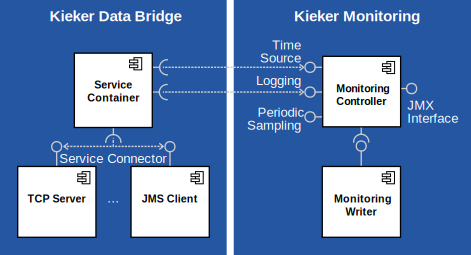
\includegraphics[width=\textwidth]{images/kieker-data-bridge}
\end{figure}
\end{frame}

% FRAME
\begin{frame}[fragile]
\frametitle{Service Connectors}
\structure{TCP Client}  Connects to a remote service on startup
\vskip1em
\structure{TCP Single Server}  Listens for one client
\vskip1em
\structure{TCP Multi Server}  Handles multiple clients
\vskip1em
\structure{JMS Client}  Connects to a JMS queue
\vskip1em
\structure{JMS Embedded}  Start a JMS service and connects to it
\end{frame}

% FRAME
\begin{frame}[fragile]
\frametitle{Service Container}
\structure{Input}
\begin{itemize}
\item Kieker Configuration
\item Service Connector
\end{itemize}
\vskip1em
\structure{Main Loop}
\begin{enumerate}
\item Setup Kieker
\item Setup service connector
\item Get record
\item goto 3 if not terminated
\item Close service connector
\item Shutdown Kieker
\end{enumerate}
\end{frame}

% FRAME
\begin{frame}[fragile]
\frametitle{Service Container}
\structure{Other Features}
\begin{itemize}
\item Connector respawn
\item Progress monitor support
\item Load record types at startup
\item Embeddable container
\end{itemize}
\end{frame}

% FRAME
\begin{frame}[fragile]
\frametitle{Service Implementations}
\structure{CLI Server}
\begin{itemize}
\item Command line application
\item Read class id mapping from ASCII file
\item Can run as deamon
\end{itemize}
\vskip1em
\structure{Eclipse Plugin}
\begin{itemize}
\item Eclipse job \& run configuration
\item Class mapping setup in run configuration
\end{itemize}
\end{frame}

% FRAME
\begin{frame}[fragile]
\frametitle{Serialization Format}
\structure{General Structure}
\begin{itemize}
\item First value \textbf{type id} (int32)
\item Other values in order of declaration
\begin{description}
\item[Kieker ] fields expressed in TYPES
\item[Other ] reflection API (non static fields)
\end{description}
\end{itemize}
\vskip1em
\structure{References}
\begin{itemize}
\item Id only
\begin{itemize}
\item First byte = 0
\item Second value \textbf{type id} (int32)
\item Unique object run-time id
\end{itemize}
\item Containment
\begin{itemize}
\item First byte = 1
\item Second value \textbf{type id} (int32)
\item Other values in order of declaration (Java only)
\end{itemize}
\end{itemize}
\end{frame}

% FRAME
\begin{frame}[fragile]
\frametitle{Serialization Format}
\structure{Binary Format}
\begin{itemize}
\item Based on \textbf{Java base-types}
\item Byte order \textbf{big endien} (network byte order)
\item String composed of
\begin{description}
\item[length ] 32bit signed integer (int)
\item[data ] variable length byte vector
\end{description}
\end{itemize}
\vskip1em
\structure{Text Format}
\begin{itemize}
\item Semicolon separated value list
\end{itemize}
\end{frame}

% FRAME
\begin{frame}[fragile]
\frametitle{Service Connector API}
\begin{lstlisting}[linebackgroundcolor={\btLstHL<2>{3,4}\btLstHL<3>{6,7}\btLstHL<4>{9,10}},escapechar=@,language=Java]
public interface IServiceConnector {

	/** setup connector */
	void setup() throws Exception;

	/** close connector */
	void close() throws Exception;

	/** get next record */
	IMonitoringRecord deserialize() throws Exception;
}
\end{lstlisting}
\end{frame}



%%
\section{Instrumentation Language}

% FRAME
\begin{frame}[fragile]
\frametitle{Instrumentation Language}
\uncover<1->{\structure{Goals}
\begin{itemize}
\item Language independent record notation
\item Annotate nodes of arbitrary models/ASTs
\end{itemize}
}
\uncover<2->{\vskip1em
\structure{Requirements}
\begin{itemize}
\item Source language meta model independent
\item Define probes for meta-model classes (nodes)
\item Define annotations (like AspectJ)
\end{itemize}
}
\end{frame}

% FRAME
\begin{frame}[fragile]
\frametitle{Language Features}
\structure{Generation of}
\begin{itemize}
\item Type compatible record types across languages
\item Serialization functions
\end{itemize}
\vskip1em
\structure{Supports}
\begin{itemize}
\item Java (example generator, run-time environment present)
\item C (example probe code)
\item Perl (example probe code)
\end{itemize}
\end{frame}

% FRAME
\begin{frame}[fragile]
\frametitle{Language Independent Record Notation}
\begin{lstlisting}[escapechar=@,language=idl]
package kieker.common

record OperationExecutionRecord {
   default string NO_SESSION_ID = "<no-session-id>"
   default long NO_TRACEID = -1
   default long NO_HOSTNAME = "<default-host>"
   default long NO_TIMESTAMP = -1
   default int NO_EOI_ESS = -1

   string operationSignature
   string sessionId = NO_SESSION_ID
   long traceId = NO_TRACEID
   long tin
   long tout
   string hostname = NO_HOSTNAME
   int eoi = NO_EOI_ESS
   int ess = NO_EOI_ESS
}
\end{lstlisting}
\end{frame}

% FRAME
\begin{frame}[fragile]
\frametitle{Language Independent Probe Notation}
\begin{lstlisting}[escapechar=@,language=ial]
package kieker.common

model java "http://www.eclipse.org/JvmTypes"

import kieker.common.OperationExecutionRecord

probe OperationExecutionProbe : java::MethodDeclaration {
   use OperationExecutionRecord
}
\end{lstlisting}
\end{frame}

% FRAME
\begin{frame}[fragile]
\frametitle{Weaver}
\structure{Weaver Technologies}
\begin{itemize}
\item AspectJ
\item Perl-Weaver (Nis)
\item AspectC or other C weaver
\end{itemize}
\vskip1em
\structure{Question}  Do we need a generic weaving language?
\end{frame}



%%
\section{Conclusion}

% FRAME
\begin{frame}[fragile]
\frametitle{Summary}
\begin{itemize}
\item Kieker Data Bridge
\begin{itemize}
\item Multi protocol support
\item Serialization method
\item Extendable record library
\item Two use cases in Perl and C
\end{itemize}
\end{itemize}
\begin{itemize}
\item Instrumentation Language
\begin{itemize}
\item Platform independent record notation
\item Generator for Java (experimental)
\end{itemize}
\end{itemize}
\end{frame}

% FRAME
\begin{frame}[fragile]
\frametitle{To Do List}
\begin{itemize}
\item Kieker Data Bridge
\begin{itemize}
\item Improve documentation
\item Refactor to meet Kieker package naming
\item Integrate into Kieker distribution
\item Support for adaptive monitoring
\item Support for AJAX/HTTP connection
\end{itemize}
\end{itemize}
\begin{itemize}
\item Instrumentation Language
\begin{itemize}
\item Finalize grammar (checks and type evaluation)
\item Generator for Perl \& C
\item Finalize generator for Java
\end{itemize}
\end{itemize}
\begin{itemize}
\item Kieker
\begin{itemize}
\item C run-time library and instrumentation (thesis)
\item Perl run-rime package
\end{itemize}
\end{itemize}
\end{frame}



%%
\section{References}

%%%%%%%%%%%%%%%%%%%%%%%%%%%%%%%%%
%\begin{frame}[t,allowframebreaks]{References}
%  \setbeamertemplate{bibliography item}[text]
%  \footnotesize
%  \bibliography{../paper/lniguide,../paper/emftext}
%\end{frame}


\end{document}
